\documentclass[preprint,12pt]{elsarticle}

\usepackage{amsmath,amssymb}
\usepackage{booktabs,longtable,array}
\usepackage{graphicx}
\usepackage{hyperref}
\usepackage{microtype}
\usepackage{xcolor}
\usepackage{seqsplit}
\providecommand{\tightlist}{\setlength{\itemsep}{0pt}\setlength{\parskip}{0pt}}
\providecommand{\pandocbounded}[1]{#1}
\newcolumntype{P}[1]{>{\raggedright\arraybackslash}p{#1}}
\setlength{\emergencystretch}{3em}
\hypersetup{hidelinks}

\journal{[Journal Name]}

\begin{document}
\sloppy
\begin{frontmatter}

\title{A Physics-Aware Benchmark for Phase-Resolved Neural Operator
Learning in Boiling Flows: Statistically Rigorous Evidence for
Condition-Dependent Architecture Trade-offs}
\author{[Author information required]}
\address{[Affiliation required]}

\begin{abstract}
Neural surrogates for boiling flows must forecast smooth thermal
structure, sharp liquid-vapor interfaces, and locally conservative
transport over long autoregressive horizons. We introduce a
reproducible, statistically rigorous benchmark for this task and use it
to show that architecture rankings for phase-resolved boiling
forecasting are highly condition-dependent --- a finding with direct
implications for how the field should evaluate operator-learning claims
going forward. On a fixed tutorial-scale trajectory split, a
Tucker-factorized Fourier Neural Operator (T-FNO) and a
parameter-comparable U-Net exhibit a statistically significant Pareto
trade-off (paired bootstrap intervals, exact sign-flip tests,
Holm-Bonferroni correction, n=11 seeds): T-FNO is significantly better
on interface-temperature fidelity, U-Net is significantly better on
mass-conservation error. When this same comparison is repeated on two
independently held-out physical conditions from the same source dataset,
however, the trade-off does not reproduce: U-Net is descriptively
favored over T-FNO on every primary metric, including interface
temperature, though the five-seed independent test is statistically
underpowered. A predeclared spectral divergence-penalty loss, applied to
a local-global hybrid architecture, restores mass-conservation
non-inferiority to U-Net on the original split (p=.000488) and transfers
the conservation advantage directionally to the independent conditions,
though not yet with confirmatory statistical power there. We
additionally identify and correct a previously unreported evaluation
pitfall --- phase-indicator (vapor-fraction) predictions exceeding their
physical {[}0,1{]} range during autoregressive rollout, which we show
can materially confound downstream interface and dry-area diagnostics
--- and demonstrate a predeclared statistical decision-gate methodology
that correctly rejects a promising but non-replicating single-seed
observation. A critical-heat-flux (CHF)-motivated heater-adjacent
dry-area proxy is evaluated across all trajectories but reveals no
sustained ground-truth event in any of them, so no claim of validated
CHF detection is made. We contribute the benchmark protocol, the
physical-validity check, the decision-gate methodology, and --- as the
central empirical finding --- direct evidence that single-condition
architecture comparisons in this domain risk reporting a property of the
test trajectory rather than a genuine architectural property, with a
concrete demonstration of how to detect this via independent-condition
replication.
\end{abstract}

\begin{keyword}
neural operator \sep Fourier neural operator \sep pool boiling \sep phase-resolved forecasting \sep conservation laws \sep BubbleML
\end{keyword}

\end{frontmatter}

\emph{Release manuscript source. The bibliography entries in the
generated manuscript were checked against the primary records documented
in \texttt{BIBLIOGRAPHY\_VERIFICATION.md}. This public artifact has no
repository URL or DOI because neither has been verified; author
metadata, if required for journal submission, must be supplied and
approved by the authors.}

\begin{center}\rule{0.5\linewidth}{0.5pt}\end{center}

\begin{center}\rule{0.5\linewidth}{0.5pt}\end{center}

\section*{1. Introduction}\label{1-introduction}

Pool boiling is one of the most effective heat transfer mechanisms
available to engineers, and it is the mechanism of last resort for the
industries that most need it: high-power electronics cooling,
data-center thermal management, and nuclear thermal-hydraulics all rely
on boiling to move heat fluxes that single-phase convection cannot
handle. The mechanism\textquotesingle s effectiveness is bounded by the
critical heat flux (CHF) --- the point at which a growing vapor film
insulates the heated surface from the liquid coolant, causing a runaway
temperature excursion that can destroy the hardware it was meant to
protect. Classical correlations for CHF (e.g., Zuber\textquotesingle s
hydrodynamic instability model) provide efficient aggregate estimates
but do not resolve the transient, spatially local bubble dynamics that
precede an actual event on a specific surface.

High-fidelity interface-tracking computational fluid dynamics (CFD) can
resolve bubble nucleation, growth, coalescence, and departure, but its
cost limits repeated design exploration and real-time digital-twin use.
Operator learning offers a route to fast state-to-state surrogates
learned directly from CFD trajectories. The Fourier Neural Operator
(FNO) is an attractive candidate because it represents global spatial
coupling through a resolution-invariant spectral representation. Boiling
fields, however, combine non-periodic domain boundaries with a sharp,
near-discontinuous liquid-vapor interface --- properties in tension with
FNO\textquotesingle s implicit periodicity assumption and its
low-frequency spectral truncation. The BubbleML benchmark reported that
a vanilla FNO underperforms a U-Net on pool-boiling temperature
forecasting by roughly a factor of two in boundary RMSE (not the
order-of-magnitude gap sometimes assumed in early framing of this
problem), attributed tentatively to convolutional edge sensitivity
versus the Fourier layer\textquotesingle s periodicity assumption.

This motivates a natural question: do parameter-efficient FNO variants
close this gap on the full, phase-resolved multi-field boiling state
(not just temperature), and --- critically --- \textbf{is any observed
architecture ranking a genuine, generalizable property of the
architectures, or an artifact of the specific trajectory it was measured
on?} The second half of this question is, to our knowledge, not
systematically addressed in prior boiling-operator benchmark work, which
typically reports single-trajectory or single-seed comparisons. We treat
it as a first-class experimental question rather than an assumed
non-issue.

This paper makes five contributions:

\begin{enumerate}
\def\labelenumi{\arabic{enumi}.}
\tightlist
\item
  A reproducible, physics-aware benchmark protocol for five-field
  (velocity, pressure gradient, temperature, vapor-phase indicator)
  phase-resolved boiling forecasting, evaluated with paired bootstrap
  intervals, exact sign-flip tests, and Holm-Bonferroni correction
  across multiple seeds.
\item
  Identification and correction of a previously unreported evaluation
  pitfall: phase-indicator predictions exceeding their physical
  {[}0,1{]} range under autoregressive rollout, and a demonstration that
  this materially confounds downstream evaluation metrics that depend on
  the phase field.
\item
  A predeclared statistical decision-gate methodology, demonstrated
  concretely by its correct rejection of a promising but non-replicating
  single-seed rollout observation --- a discipline we argue should be
  standard practice before committing engineering effort to an observed
  effect.
\item
  \textbf{A cross-condition replication check}, in which a statistically
  confirmed architecture trade-off (T-FNO favors interface fidelity,
  U-Net favors mass conservation) on one trajectory split is directly
  re-tested on two independently held-out physical conditions from the
  same source dataset --- and does not reproduce. We present this not as
  a disappointing result but as the paper\textquotesingle s central
  empirical and methodological contribution: direct, controlled evidence
  that single-condition benchmarking in this domain can report an
  artifact of the test trajectory.
\item
  A predeclared, mechanistically motivated conservation intervention (a
  spectral velocity-divergence penalty) that restores mass-conservation
  non-inferiority to U-Net on the original split and transfers the
  conservation advantage directionally --- though not yet confirmatorily
  --- to the independent conditions, illustrating how a targeted
  physical constraint, rather than architecture complexity alone, is
  needed to move a specific objective.
\end{enumerate}

Consistent with contribution 4, our central finding is not a single
winning architecture. It is that \textbf{architecture rankings for
phase-resolved boiling forecasting are condition-dependent}, and that
reporting a ranking from a single trajectory --- however statistically
rigorous the seed-level inference --- is not sufficient evidence of a
generalizable architectural property. We view this as a methodological
finding of independent value to the broader neural-operator-for-science
community, beyond its specific application to boiling.

\begin{center}\rule{0.5\linewidth}{0.5pt}\end{center}

\section*{2. Related Work}\label{2-related-work}

\subsection*{2.1 Classical CHF prediction and boiling
simulation}\label{21-classical-chf-prediction-and-boiling-simulation}

Critical heat flux has been studied mechanistically since the
mid-twentieth century, most influentially through
Zuber\textquotesingle s hydrodynamic instability model\cite{zuber1959hydrodynamic}. Engineering
practice also uses application-specific correlations for CHF estimation.
These are computationally simple aggregate predictors, but they do not
resolve transient local bubble dynamics on a specific surface and offer
no natural mechanism for real-time, sensor-driven early warning.

Direct numerical resolution of boiling requires interface-tracking
methods --- volume-of-fluid, level-set, or phase-field formulations
coupled to the Navier-Stokes and energy equations. The BubbleML dataset\cite{hassan2023bubbleml},
which underlies the present work\textquotesingle s data, was generated
with the Flash-X interface-tracking solver and spans multiple fluids,
heater geometries, and boiling regimes. Its accompanying benchmark paper
is, to our knowledge, the first systematic comparison of neural operator
architectures against convolutional baselines on boiling data, and its
reported \textasciitilde2x FNO-versus-U-Net temperature BRMSE gap is the
empirical starting point for the present investigation.

\subsection*{2.2 Operator learning and convolutional
surrogates}\label{22-operator-learning-and-convolutional-surrogates}

The Fourier Neural Operator\cite{li2021fno} performs global convolution via pointwise
multiplication in a truncated Fourier domain, and has demonstrated
strong performance on smooth, largely periodic PDE systems.
Convolutional U-Net architectures\cite{ronneberger2015unet} instead rely on local receptive fields
and multi-scale skip connections, and serve as a strong general-purpose
baseline for dense spatial prediction, including PDE surrogate modeling.

Several parameter-efficient FNO variants address the capacity and
generalization trade-offs of the original architecture.
Tensor-factorized (Tucker) FNO represents the spectral weight tensor in
a low-rank Tucker decomposition; axis-factorized FNO (F-FNO)\cite{tran2023ffno} factorizes
the spectral convolution along each spatial axis independently. The
BubbleML benchmark\textquotesingle s own results indicate both variants
outperform vanilla FNO on boiling forecasting despite having
substantially fewer parameters, attributed to reduced overfitting to
excess spectral capacity rather than a fix to the underlying periodicity
or discontinuity issue. U-shaped FNO (UNO)\cite{rahman2022uno} grafts U-Net-style
multi-scale structure onto Fourier blocks; the LOGLO-FNO family of
Kalimuthu et al. (2025)\cite{kalimuthu2025loglo} explicitly combines local and global spectral
branches to improve local, high-frequency representation.
Transformer-based operators, including a recent boiling-specific
transformer forecaster (Bubbleformer\cite{hassan2025bubbleformer}) benchmarked on the extended
BubbleML 2.0 release, represent a further active direction ---
indicating this remains a contested design space rather than a settled
one. None of these architecture families, to our knowledge, has been
evaluated with an explicit cross-condition replication check of the kind
this paper performs. Hard-constrained alternatives to the present soft
divergence penalty include the continuity-by-construction networks of
Richter-Powell et al. (2022)\cite{richterpowell2022neural} and the differentiable spectral Leray
projection used by Li et al. (2026)\cite{li2026project}; neither is evaluated here on
phase-resolved boiling.

\subsection*{2.3 Experimental boiling
diagnostics}\label{23-experimental-boiling-diagnostics}

Independent of the simulation-data operator-learning literature,
Ravichandran et al. (2021)\cite{ravichandran2021decrypting} used high-resolution infrared thermometry to
investigate boiling-crisis diagnostics, and Ravichandran et al. (2023)\cite{ravichandran2023dryareas}
developed online dry-area detection from infrared measurements using
deep learning. This experimental line of work and the simulation-based
operator-learning line of work reviewed above remain largely disjoint;
no result in the present paper establishes transfer to experimental
measurements or deployment-grade CHF warning.

\subsection*{2.4 Reproducibility and the gap
addressed}\label{24-reproducibility-and-the-gap-addressed}

Open boiling datasets are fragmented across repositories, fields, grids,
regimes, and evaluation conventions, a fragmentation documented by
Dunlap et al. (2026)\cite{dunlap2026open} in their survey of open multimodal thermal-fluid
datasets and software. This work\textquotesingle s explicit,
checksum-verified data and evaluation pipeline is designed to partially
mitigate this within its own declared artifact boundary. Combined with
the cross-condition replication check described above, we position this
work primarily as a benchmark and evaluation-methodology contribution
--- a genuinely rigorous protocol for making and testing architecture
claims on chaotic, multiphysics surrogate tasks --- rather than as a
claim of a novel architecture. The individual architectural components
used here (Tucker/factorized FNO, local-global hybridization, spectral
divergence penalties, bounded output heads) are each drawn from or
closely related to existing techniques; the contribution is their
careful, statistically disciplined integration and, specifically, the
demonstration that even a well-powered single-condition comparison among
them is not sufficient evidence of a generalizable ranking.

{\def\LTcaptype{none} % do not increment counter
\begin{longtable}[]{@{}P{0.22\textwidth}P{0.58\textwidth}P{0.14\textwidth}@{}}
\toprule\noalign{}
Feature & BubbleML (original) & This work \\
\midrule\noalign{}
\endhead
\bottomrule\noalign{}
\endlastfoot
Multiple trajectories & Yes (79 simulated conditions) & Yes \\
Interface and conservation metrics jointly reported & Not reported for
the neural-PDE benchmark & Yes \\
Multi-seed paired statistical testing & Not reported & Yes (n=11
tutorial; n=5 cross-condition) \\
Cross-condition architecture replication & Not reported; the paper
reports heat-flux holdout cross-validation & Yes \\
Physical output-validity enforcement & Not reported & Yes (bounded-alpha
head) \\
Predeclared decision gates & Not reported & Yes \\
Artifact release & Partial (data, code, and model zoo reported) &
Partial (stored-result self-test; raw data/checkpoints remain
external) \\
\end{longtable}
}

\emph{Table 1. Protocol comparison. ``Not reported'' indicates that the
original BubbleML paper does not document the feature for its neural-PDE
benchmark; it does not establish absence.}

\begin{center}\rule{0.5\linewidth}{0.5pt}\end{center}

\section*{3. Methods}\label{3-methods}

\subsection*{3.1 Data, preprocessing, and
splits}\label{31-data-preprocessing-and-splits}

\textbf{Tutorial-scale split.} The primary comparison uses three
official downsampled Pool-Boiling Subcooled FC-72 examples at 48×48
resolution, preprocessed into PyTorch tensors with no synthetic
fallback. The trajectory-level split prevents temporal leakage:
Twall-103 is train, Twall-106 is validation, and Twall-100 is test. Each
source has 169 released-grid frames, yielding 160 valid
five-history/five-future temporal windows per split.

{\def\LTcaptype{none} % do not increment counter
\begin{longtable}[]{@{}P{0.25\textwidth}P{0.55\textwidth}P{0.14\textwidth}@{}}
\toprule\noalign{}
Source & SHA-256 & Role \\
\midrule\noalign{}
\endhead
\bottomrule\noalign{}
\endlastfoot
\texttt{Twall-103.hdf5} &
\texttt{\seqsplit{25b305661dee59cf5df49eb2563a4ed08f79664ba377e57877fcda5a948956dd}}
& train \\
\texttt{Twall-106.hdf5} &
\texttt{\seqsplit{4308e5be884c3edcf301e9c12bff8d499d53729be3820aa18e255a5152fbd004}}
& validation \\
\texttt{Twall-100.hdf5} &
\texttt{\seqsplit{5bf2539628c3595f39517c466f6971da76f137358771592c14ad1a5881e4d1bf}}
& test / rollout \\
\end{longtable}
}

The released fields are time×y×x grids; row 0 is immediately above the
heater; physical boundary cells are omitted. Reported outer-grid
quantities are therefore interior-edge proxies, not wall residuals.

\textbf{Independent multi-trajectory split.} The cross-condition
replication check uses the official ten-trajectory, native 384×384
Pool-Boiling Subcooled legacy archive (SHA-256
\texttt{\seqsplit{2eba140d74cbb7b01a55f0684227dea94306aea516a0f864831485d31d25f655}};
201 frames/trajectory; Twall 79, 81, 85, 90, 95, 98, 100, 103, 106,
110). Trajectory roles were frozen before any model training or test
inspection: train on Twall 79, 85, 90, 95; validate on Twall 81; test
independently on Twall 98 and Twall 110. Twall 100, 103, and 106 were
excluded, since they form the tutorial split. Continuous fields were
bilinearly downsampled to 96×96; the binary phase mask used
nearest-neighbor downsampling; physical grid spacings were rescaled
consistently. After discarding source frames 0--29, each trajectory
contributes 170 frame records, yielding 644/161/322 valid windows for
train/validation/test. A separate one-epoch, batch-size-one feasibility
check was also run at native 384×384 resolution to test direct execution
and memory feasibility only (not convergence or ranking).

\pandocbounded{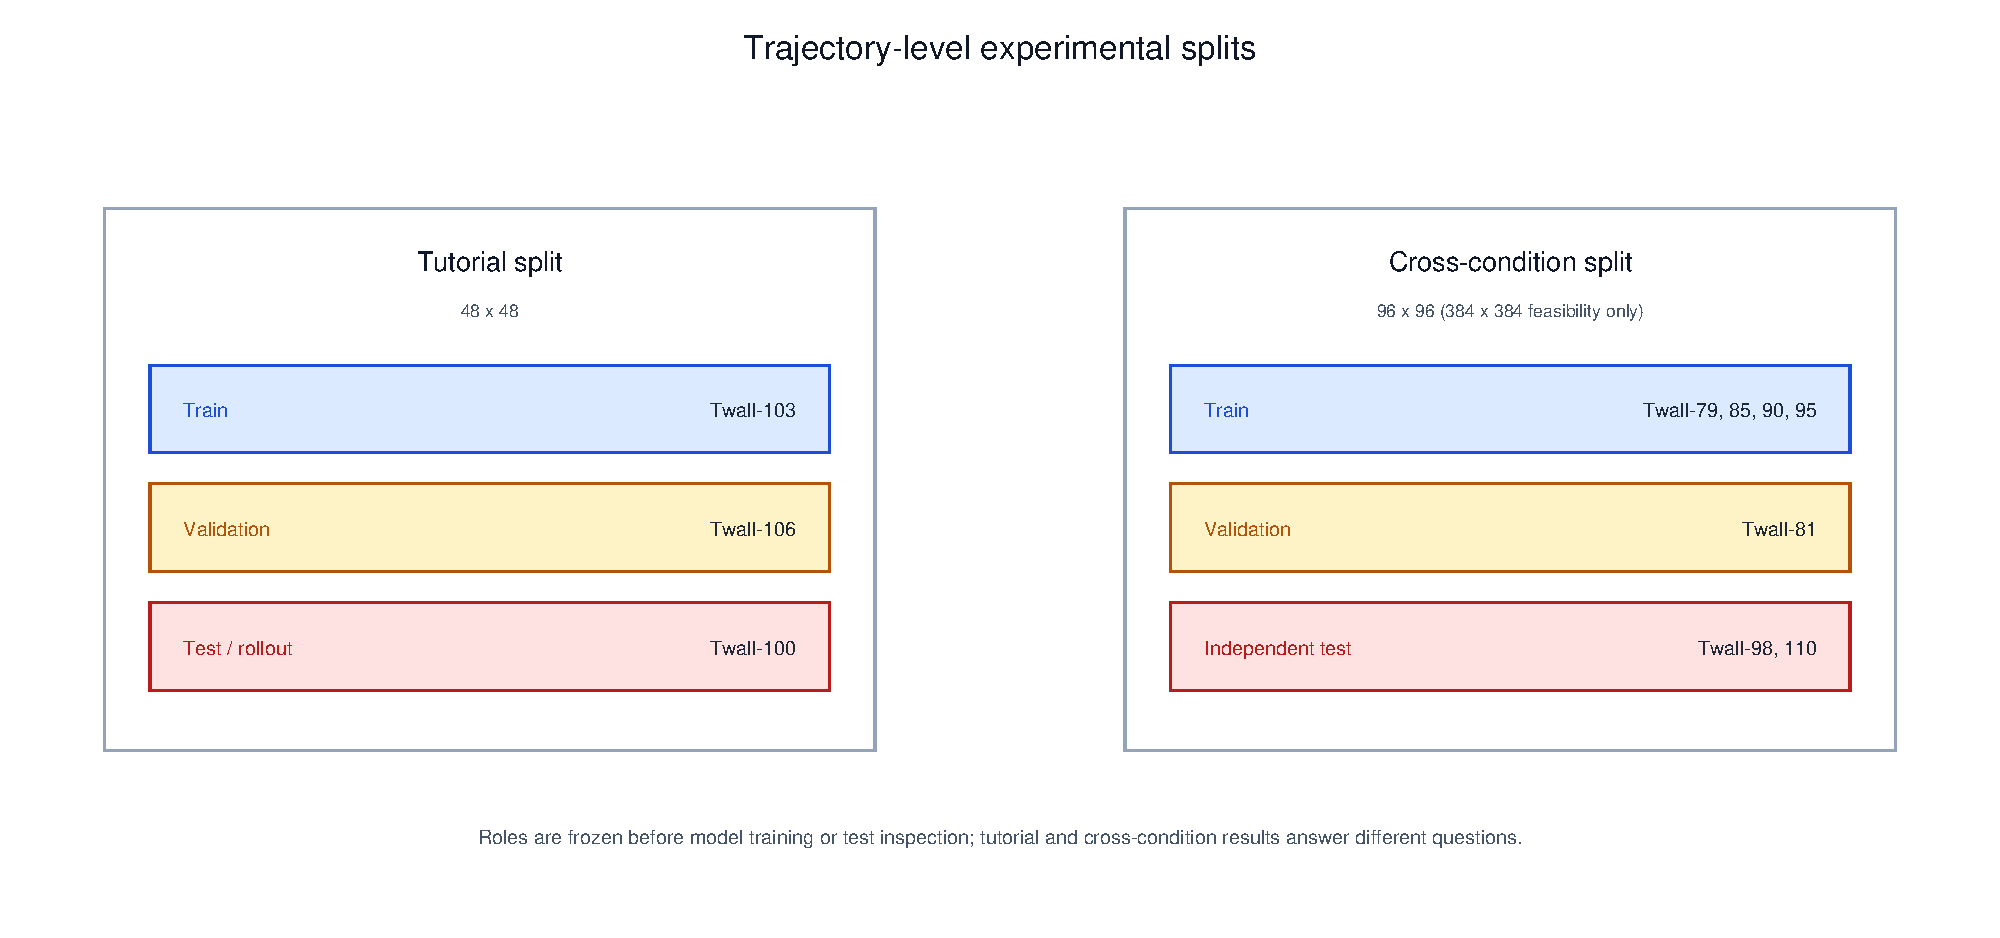
\includegraphics[width=\linewidth]{../submission/figures/fig6_split_design.pdf}}

\textbf{Figure 2.} The tutorial split evaluates a fixed three-trajectory
comparison; the independent cross-condition split directly tests
transfer of that comparison to two held-out conditions. The roles were
frozen before training or test inspection.

\subsection*{3.2 Model architectures and training
protocol}\label{32-model-architectures-and-training-protocol}

Four base models are compared: vanilla FNO, Tucker-factorized FNO
(T-FNO, rank 0.1), axis-factorized FNO (F-FNO)\cite{tran2023ffno}, and a
parameter-comparable U-Net. Each uses five history and five forecast
frames (25 input/output channels), AdamW (lr 1e-3, weight decay 0.01),
batch size 8, horizontal reflection augmentation, global gradient-norm
clipping at 1.0, and training to a predeclared two-window
validation-plateau stopping rule (200-epoch ceiling). Fourier-family
models train at full 48×48 (tutorial) or 96×96 (cross-condition)
resolution with 24×24 real-FFT modes --- the maximum representable given
the Nyquist limit at these resolutions (max unique modes = N/2 + 1),
correcting an earlier invalid 64-mode configuration that would have
silently collapsed under half-resolution training.

The tutorial-split four-model comparison used seeds 42, 100, 1234, 2025,
9999; a disclosed six-seed T-FNO/U-Net extension added seeds 7, 17, 314,
2718, 4242, 7777, for 11 paired seeds total. The cross-condition
comparison used seeds 42, 100, 1234, 2025, 9999 (n=5) on an actual
NVIDIA Tesla T4 via CUDA; tutorial-split runs used an Apple M2 via Metal
Performance Shaders (MPS). With five paired seeds, the minimum
attainable two-sided exact sign-flip p-value is 0.0625; direction and
interval width, not corrected significance, are the primary evidence at
this sample size.

\subsection*{3.3 Physical output-bounding for the phase
indicator}\label{33-physical-output-bounding-for-the-phase-indicator}

Unconstrained models produced decoded vapor-fraction (alpha) predictions
outside the physical {[}0,1{]} interval during autoregressive rollout
(observed ranges up to {[}-0.157, 1.408{]}). We correct this at the
model level: writing the raw normalized-space alpha logit as
\(z_\alpha\), and \(a_0, a_1\) as the normalized coordinates that decode
to physical alpha 0 and 1 respectively, the bounded output is

\[
\widehat{\alpha}_N = a_0 + (a_1 - a_0)\,\sigma(z_\alpha), \qquad \widehat{\alpha} = \operatorname{decode}(\widehat{\alpha}_N) \in [0,1]. \tag{1}
\]

All non-alpha channels remain unconstrained. This guarantees physical
validity by construction, without post-hoc clipping of autoregressively
fed-back predictions.

\subsection*{3.4 Local-global hybrid
architecture}\label{34-local-global-hybrid-architecture}

For hybrid layer \(\ell\), the local-global composition adds a learned
local convolution branch in parallel with the spectral and
pointwise-residual paths:

\[
z^{(\ell+1)} = \phi\!\left(\mathcal{K}^{(\ell)}_{\text{Tucker}}z^{(\ell)} + \mathcal{C}^{(\ell)}_{3\times 3}z^{(\ell)} + W^{(\ell)}z^{(\ell)}\right), \tag{2}
\]

where \(\mathcal{K}_{\text{Tucker}}\) is the truncated Tucker-factorized
spectral convolution, \(\mathcal{C}_{3\times3}\) is a learned 3×3 local
convolution, \(W\) is the pointwise residual map, and \(\phi\) is the
layer nonlinearity. This architecture was motivated specifically by the
confirmed tutorial-split Phase 1 Pareto trade-off (Section 4.1) --- a
predeclared statistical decision gate (Section 3.6) had separately and
correctly rejected an earlier, unrelated intervention aimed at a
non-replicating single-seed rollout artifact; the two are distinct and
should not be conflated.

\subsection*{3.5 Conservation-targeted divergence
penalty}\label{35-conservation-targeted-divergence-penalty}

The conservation intervention augments the local-global
hybrid\textquotesingle s training objective with a spectral
velocity-divergence penalty, computed on decoded physical-coordinate
velocity to avoid spatial discretization error:

\[
\mathcal{L} = \mathcal{L}_{\text{data}} + \lambda_{\text{div}} \cdot \frac{1}{BTHW}\sum_{b,t,x,y} \left| \mathcal{F}^{-1}\!\left[ i k_x \mathcal{F}(u_{b,t}) + i k_y \mathcal{F}(v_{b,t}) \right]_{x,y} \right|, \tag{3}
\]

using each sample\textquotesingle s physical grid spacings for the
wavenumbers \(k_x, k_y\). Validation data MSE remains the
checkpoint-selection criterion; \(\lambda_{\text{div}}\) was selected in
two stages, described fully in Section 4.3, to avoid conflating
hyperparameter selection with confirmatory evaluation.

\subsection*{3.6 Statistical protocol and decision
gates}\label{36-statistical-protocol-and-decision-gates}

All architecture and intervention claims use paired, multi-seed
inference: a deterministic 10,000-sample paired bootstrap for confidence
intervals, an exact paired sign-flip test for significance, and
Holm-Bonferroni correction across the full family of metrics tested in a
given comparison. An earlier statistical audit corrected two
implementation details --- removing an unnecessary Monte Carlo add-one
correction from the exact sign-flip enumeration, and excluding
compute-only (non-error) metrics from the Holm family --- and all
numbers reported in Section 4 reflect the corrected implementation.

Architectural interventions are evaluated under \textbf{predeclared
decision gates}: a fixed statistical criterion (non-inferiority margin,
significance threshold, and metric family) is frozen before training and
evaluation, and the intervention is only reported as successful if the
frozen criterion is met. This discipline was demonstrated concretely
when an initial single-seed pair showed a promising reversal in rollout
dry-area tracking after the phase-bounding fix (Section 3.3); a
predeclared 11-seed confirmatory test showed this reversal did not
replicate (Section 4.2), and the corresponding architectural
interventions were correctly not pursued on that basis. The local-global
hybrid (Section 3.4) and divergence penalty (Section 3.5) are motivated
by a separate, independently confirmed finding (the tutorial-split
Pareto trade-off) and are not affected by that earlier
gate\textquotesingle s rejection.

\subsection*{3.7 CHF-motivated autoregressive proxy
evaluation}\label{37-chf-motivated-autoregressive-proxy-evaluation}

A fully autoregressive evaluator feeds each model\textquotesingle s own
five-frame predictions back as input for the next step (no ground-truth
injection), producing long rollouts from a short seed history. The
CHF-motivated proxy signal is the fraction of heater-adjacent cells
(rows 0:4) with predicted alpha \textgreater{} 0.5. The event threshold
is
\(\max(0.10, \text{median of first 20 ground-truth forecast frames} + 0.10)\),
requiring three consecutive frames at or above threshold to count as a
sustained precursor. This is an illustrative phase-based proxy, not a
calibrated CHF label: none of the available trajectories has a
synchronized wall-heat-flux series or an independently verified
stable-to-CHF transition.

\pandocbounded{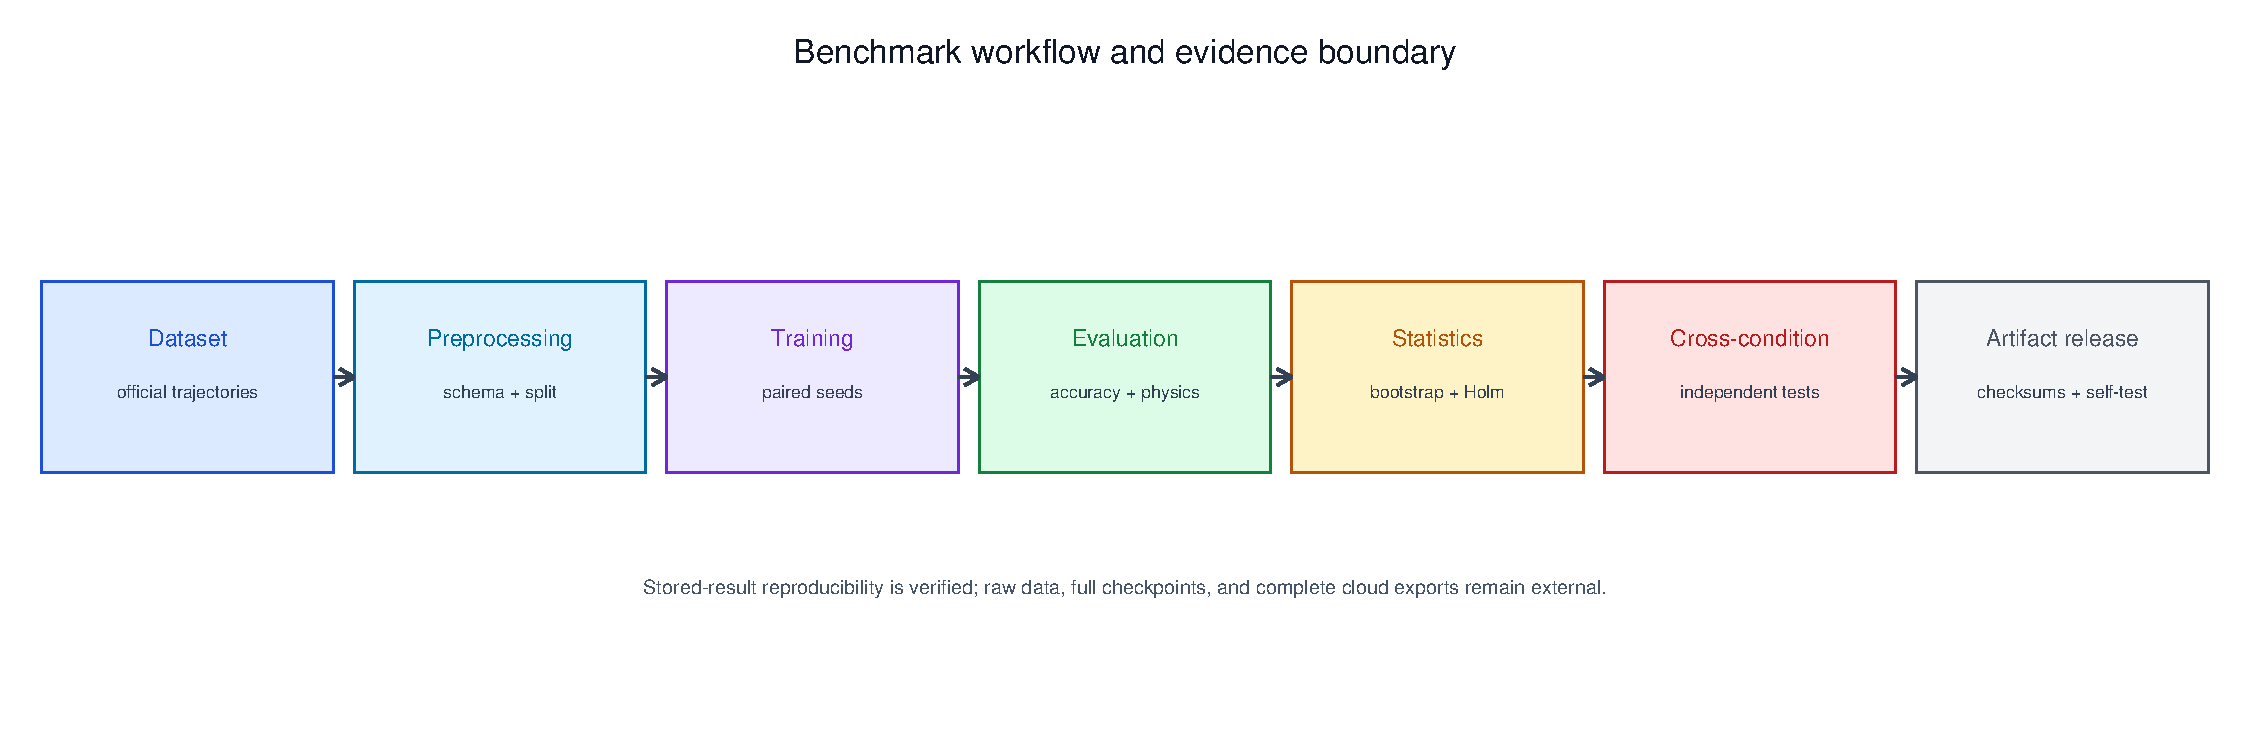
\includegraphics[width=\linewidth]{../submission/figures/fig5_benchmark_workflow.pdf}}

\textbf{Figure 3.} Benchmark workflow. The last transition makes the
artifact boundary explicit: the stored-result statistical self-test is
reviewer-runnable, while raw data, full checkpoints, and complete
cloud-side cross-condition exports remain external.

\begin{center}\rule{0.5\linewidth}{0.5pt}\end{center}

\section*{4. Results}\label{4-results}

\subsection*{4.1 Tutorial split: T-FNO and U-Net form a statistically
confirmed Pareto
trade-off}\label{41-tutorial-split-t-fno-and-u-net-form-a-statistically-confirmed-pareto-trade-off}

Across 11 paired seeds, no overall GWRMSE winner was established (T-FNO
− U-Net: −0.05698, 95\% paired bootstrap CI {[}−0.12314, +0.00946{]},
sign-flip p=.1469, Holm p=1.0). T-FNO was significantly better on
interface-temperature RMSE (−0.50190, Holm p=.0352) and
interface-temperature-jump MAE (−0.43147, Holm p=.0215), but
significantly worse on mass-conservation MAE (+0.04494, Holm p=.0215).

\subsection*{4.2 Physical validity is an evaluation requirement,
independent of architecture
ranking}\label{42-physical-validity-is-an-evaluation-requirement-independent-of-architecture-ranking}

Unbounded models produced physically invalid alpha values under rollout
({[}−0.157, 1.408{]} for T-FNO, {[}−0.108, 1.417{]} for U-Net over 164
steps). The output-head fix (Eq. 1) constrained both to {[}0,1{]} by
construction. An initial single-seed comparison after this fix showed a
large reversal in cumulative dry-area tracking error (bounded T-FNO
0.12167 vs. bounded U-Net 0.05275); a predeclared 11-seed confirmation,
however, found this did not replicate as a significant effect (paired
difference +0.00775, 95\% CI {[}−0.00393, +0.01829{]}, Holm p=1.0 across
all 21 tested rollout metrics, smallest adjusted p=0.3997). We report
this explicitly as a methodological finding: physical-validity
correction and architecture superiority are distinct questions, and
single-seed rollout observations --- even after a legitimate bug fix ---
require the same multi-seed confirmatory discipline as any other
architecture claim.

\subsection*{4.3 A local branch alone does not recover conservation; a
targeted divergence penalty does, on the tutorial
split}\label{43-a-local-branch-alone-does-not-recover-conservation-a-targeted-divergence-penalty-does-on-the-tutorial-split}

The zero-penalty local-global hybrid (Eq. 2) was tested under three
predeclared non-inferiority criteria (5\% margins from the Phase 1
comparators): non-inferior to T-FNO on interface-temperature RMSE (Holm
p=.00146) and jump MAE (Holm p=.00146, bootstrap interval favoring the
hybrid), but it \textbf{failed} mass-conservation non-inferiority to
U-Net by a wide margin (+0.03876 against a 0.00829 margin; Holm p=1.0 in
the unchanged complete-metric family, p=.02148). A local receptive field
alone does not import U-Net\textquotesingle s conservation behavior.

An initial divergence-penalty pilot (2 seeds,
\(\lambda_{\text{div}} \in \{.01, .03, .10\}\), all eligible under a 5\%
data-fit guard) selected \(\lambda_{\text{div}}=.10\); an 11-seed
confirmation passed the single predeclared mass-conservation
non-inferiority criterion (mean mass MAE 0.14499 vs.
U-Net\textquotesingle s 0.16586; paired difference −0.02086, 95\% CI
{[}−0.02845, −0.01331{]}; p=.000488), without an established interface
regression relative to the zero-penalty hybrid.

An expanded, more rigorous sensitivity sweep (3 seeds,
\(\lambda_{\text{div}} \in \{.01, .03, .10, .20, .30\}\), both a
data-fit and an interface-RMSE guard) found validation divergence
decreasing monotonically through the full tested range, with 0.30 ---
the upper tested boundary --- selected as the eligible candidate with
lowest divergence. \textbf{This selection identifies a value that works
within the tested range; it does not identify an interior optimum, and
behavior beyond 0.30 remains untested} (see Section 6, future work). A
fresh 11-seed confirmation at \(\lambda_{\text{div}}=.30\) passed the
same predeclared criterion with a substantially larger margin: mean mass
MAE 0.09373 vs. U-Net\textquotesingle s 0.16586 (paired difference
−0.07212, 95\% CI {[}−0.07940, −0.06535{]}, p=.000488), with no
established interface regression relative to the zero-penalty hybrid. We
adopt \(\lambda_{\text{div}}=.30\) as the primary divergence-hybrid
configuration for the remainder of this paper.

\subsection*{4.4 Cross-condition replication: the tutorial-split
trade-off does not reproduce (central
finding)}\label{44-cross-condition-replication-the-tutorial-split-trade-off-does-not-reproduce-central-finding}

On two independently held-out physical conditions (Twall 98, Twall 110;
n=5 paired seeds), the descriptive ranking changed substantially from
the tutorial split:

{\def\LTcaptype{none} % do not increment counter
\begin{longtable}[]{@{}P{0.20\textwidth}P{0.13\textwidth}P{0.18\textwidth}P{0.19\textwidth}P{0.16\textwidth}@{}}
\toprule\noalign{}
Model & GWRMSE & Interface-temperature RMSE & Interface-temperature-jump
MAE & Mass-conservation MAE \\
\midrule\noalign{}
\endhead
\bottomrule\noalign{}
\endlastfoot
T-FNO & 11.5974 & 14.5207 & 8.7655 & 0.12989 \\
\textbf{U-Net} & \textbf{11.5029} & \textbf{13.9057} & \textbf{8.5757} &
0.11560 \\
Local-global hybrid (zero penalty) & 11.6323 & 14.4567 & 8.7021 &
0.13583 \\
Divergence hybrid (\(\lambda_{\text{div}}=.30\)) & 11.5859 & 14.2120 &
8.6981 & \textbf{0.08669} \\
\end{longtable}
}

For T-FNO minus U-Net: GWRMSE +0.09448 (95\% CI {[}+0.04363,
+0.14534{]}), interface-temperature RMSE +0.61497 ({[}+0.31906,
+0.90941{]}), jump MAE +0.18985 ({[}+0.18080, +0.19935{]}), mass MAE
+0.01429 ({[}+0.00915, +0.02085{]}). Every unadjusted exact two-sided
p-value is .0625 (the minimum attainable at n=5) and every Holm-adjusted
p-value is 1.0. \textbf{The directions are consistent across all seeds
and both held-out trajectories, and they consistently favor U-Net ---
the opposite of the tutorial split\textquotesingle s interface-fidelity
result} --- but the five-seed design cannot establish corrected
statistical significance. We report this as a clear descriptive reversal
that current statistical power cannot confirm, not as an established new
ranking.

The divergence hybrid\textquotesingle s conservation advantage
transferred directionally: mass MAE 0.08669 vs. U-Net\textquotesingle s
0.11560 (paired difference −0.02891, 95\% CI {[}−0.03359, −0.02422{]}
relative to U-Net --- descriptive, as this specific superiority contrast
was not the split\textquotesingle s predeclared target), while remaining
descriptively worse than U-Net on GWRMSE, interface-temperature RMSE,
and jump MAE. The per-trajectory breakdown (Twall 98 and Twall 110
separately) shows the same ordering within each condition, indicating
the reversal is not driven by one anomalous trajectory, though two
conditions remain too few to characterize population-level
physical-regime variation.

\subsection*{4.5 CHF-motivated proxy: no sustained event in any available
trajectory}\label{45-chf-motivated-proxy-no-sustained-event-in-any-available-trajectory}

The dry-area proxy (Section 3.7) was evaluated on Twall-100 (tutorial
test) and, newly, on the independent Twall-98 and Twall-110
trajectories. None showed a sustained crossing: Twall-100 had 3/164
above-threshold frames (longest run 2), Twall-98 had 0/170, and
Twall-110 had 1/170 (longest run 1). No trajectory in the currently
available data supports a lead-time, sensitivity, or missed-event-rate
evaluation. This is a negative feasibility result for CHF-proxy event
evaluation with current data, not evidence about CHF predictability in
general.

\subsection*{4.6 Native-resolution feasibility and computational
cost}\label{46-native-resolution-feasibility-and-computational-cost}

One-epoch, batch-size-one runs at native 384×384 completed successfully
for all four models on the Tesla T4 (5.91--6.99s/epoch for the
Fourier-family models, 2.77s for U-Net), confirming direct execution
feasibility without establishing convergence or ranking. At the
converged 96×96 cross-condition scale:

{\def\LTcaptype{none} % do not increment counter
\begin{longtable}[]{@{}P{0.18\textwidth}P{0.21\textwidth}P{0.15\textwidth}P{0.17\textwidth}P{0.16\textwidth}@{}}
\toprule\noalign{}
Model & Parameters (stored / real-scalar) & Mean training time/seed (s)
& Inference latency (ms/window) & Throughput (windows/s) \\
\midrule\noalign{}
\endhead
\bottomrule\noalign{}
\endlastfoot
T-FNO & 548,837 / 1,040,625 & 216.09 & 4.467 & 223.94 \\
U-Net & 7,770,169 / 7,770,169 & 98.72 & 2.026 & 493.63 \\
Local-global hybrid & 696,549 / 1,188,337 & 293.45 & 5.369 & 186.25 \\
Divergence hybrid & 696,549 / 1,188,337 & 294.43 & 5.384 & 185.75 \\
\end{longtable}
}

U-Net is the fastest model to train and the lowest-latency at inference,
despite having roughly 6--14× more parameters than the FNO-family
variants --- a practical consideration alongside the
accuracy/conservation trade-offs above.

\begin{center}\rule{0.5\linewidth}{0.5pt}\end{center}

\section*{5. Discussion}\label{5-discussion}

\subsection*{5.1 Condition dependence is the central finding, not a
limitation to route
around}\label{51-condition-dependence-is-the-central-finding-not-a-limitation-to-route-around}

The tutorial-split result (Section 4.1) is real and statistically
confirmed under a rigorous multi-seed protocol. It is also, on its own,
an incomplete and potentially misleading basis for an architecture
recommendation --- a fact this paper\textquotesingle s own
cross-condition check (Section 4.4) demonstrates directly. This matters
beyond the specific T-FNO/U-Net comparison: it is evidence that
\textbf{a statistically well-powered single-trajectory comparison,
however rigorously analyzed at the seed level, does not by itself
establish a generalizable architectural property} in this domain. We
consider this the paper\textquotesingle s most transferable
contribution, of direct relevance to any future benchmark work in
phase-resolved multiphysics operator learning: seed-level rigor and
condition-level rigor are separate axes of evidence, and a benchmark
claim needs both.

A plausible, though unproven, contributing mechanism is that spectral
truncation\textquotesingle s smoothing behavior and a local receptive
field\textquotesingle s edge sensitivity trade off differently depending
on the specific interface geometry, thermal gradient magnitude, and
vapor coverage extent present in a given trajectory --- properties that
vary meaningfully with wall superheat. We note this as a candidate
explanation consistent with the observed pattern, not as an established
causal mechanism; isolating it would require a dedicated study
correlating per-trajectory physical statistics (interface curvature,
vapor coverage fraction, thermal gradient magnitude) with per-trajectory
architecture ranking, which the current two-condition independent test
cannot support.

\subsection*{5.2 The divergence penalty is the more robust of the two
interventions
tested}\label{52-the-divergence-penalty-is-the-more-robust-of-the-two-interventions-tested}

Unlike the interface/conservation ranking itself, the divergence
penalty\textquotesingle s conservation benefit transferred directionally
across both the tutorial split and the independent conditions (Sections
4.3--4.4), even though only the tutorial-split result carries full
statistical confirmation. This is consistent with the penalty targeting
a specific, physically motivated quantity (velocity divergence)
directly, rather than relying on an architectural inductive bias
(locality) whose interaction with a given trajectory\textquotesingle s
specific physical conditions is less predictable. We view this as
suggestive, not conclusive, evidence that explicit physical constraints
generalize more reliably than architectural changes alone for this class
of problem --- a hypothesis for future, better-powered testing (Section
6). The differentiable Leray-projection approach of Li et al. (2026)\cite{li2026project} is
a natural harder alternative: it constrains the velocity field to a
divergence-free subspace, whereas the present work only penalizes
divergence during training. This paper does not test that hard
constraint, and it should not be interpreted as a comparison with it.

\subsection*{5.3 Physical output validity is necessary but
architecturally
orthogonal}\label{53-physical-output-validity-is-necessary-but-architecturally-orthogonal}

The phase-bounding correction (Section 3.3) is, independent of any
architecture ranking, a requirement for trustworthy autoregressive
evaluation of any phase or volume-fraction field. The initial
single-seed reversal it produced in rollout behavior (Section 4.2) is a
cautionary example of exactly the single-condition/single-seed
over-interpretation risk this paper\textquotesingle s broader argument
(Section 5.1) warns against, now demonstrated at the seed level rather
than the trajectory level. We recommend both checks --- physical-bound
verification and multi-seed confirmation --- as standard practice for
future phase-resolved operator-learning evaluations.

\subsection*{5.4 CHF-motivated evaluation remains
proxy-only}\label{54-chf-motivated-evaluation-remains-proxy-only}

Across every trajectory available to this study, no sustained
ground-truth dry-area event was observed (Section 4.5). The dry-area
proxy therefore functions in this paper as an autoregressive-stability
stress test and a demonstration of the physical-bounding pitfall
(Section 4.2), not as an evaluation of CHF detectability, which would
require at minimum one trajectory with a verified stable-to-film-boiling
transition and, ideally, a synchronized wall-heat-flux measurement
independent of the model\textquotesingle s own output.

\subsection*{5.5 Limitations}\label{55-limitations}

{\def\LTcaptype{none} % do not increment counter
\begin{longtable}[]{@{}P{0.25\textwidth}P{0.33\textwidth}P{0.29\textwidth}@{}}
\toprule\noalign{}
Dimension & Limitation & Status in this work \\
\midrule\noalign{}
\endhead
\bottomrule\noalign{}
\endlastfoot
Statistical power, cross-condition & Independent test uses 2
trajectories, 5 seeds; minimum exact p=.0625, no Holm-significant
cross-condition result & Directionally consistent, explicitly reported
as unconfirmed \\
Physical-condition sampling & 2 held-out conditions cannot characterize
population-level regime variation & Explicitly scoped; not generalized
beyond these conditions \\
Resolution & 96×96 cross-condition training is converged; 384×384 is
feasibility-only (1 epoch) & Native-resolution convergence is future
work \\
Phase representation & Binary \texttt{dfun\textgreater{}0} mask, not
continuous volume fraction; omits surface tension/contact-angle dynamics
& Acknowledged; continuous-target ablation is future work \\
CHF validity & No trajectory contains a verified stable-to-CHF
transition or synchronized heat-flux series & Proxy-only throughout; no
detection claim made \\
Divergence-penalty selection & \(\lambda_{\text{div}}=.30\) is the upper
boundary of the tested range & Section 6 future work extends the
range \\
Conservation scope & Only velocity divergence is penalized;
energy/momentum conservation are not explicitly constrained & Noted as
an open direction \\
Architecture coverage & No comparison to transformer-based operators
(e.g., Bubbleformer) or hard-constrained conservation layers &
Explicitly out of scope this cycle; noted as related work \\
Hardware & Tutorial-split results use Apple M2/MPS; cross-condition
results use NVIDIA T4/CUDA & Both reported explicitly per experiment;
not cross-validated on identical hardware \\
Reproducibility & All data checksummed, all seeds/configs logged,
decision gates predeclared & Full artifact manifest in Section 7 \\
\end{longtable}
}

\subsection*{5.6 Practical and methodological
implications}\label{56-practical-and-methodological-implications}

For practitioners, the safest actionable guidance from this study is: do
not select an architecture for phase-resolved boiling forecasting based
on a single trajectory\textquotesingle s results, regardless of how many
seeds or how rigorous the statistical test at that trajectory. Where an
explicit conservation requirement exists, a targeted physical penalty
(Section 4.3--4.4) currently appears to be the more robust lever than
architectural locality alone, though this too awaits confirmation at
higher cross-condition statistical power. Where interface fidelity is
paramount and only a single, representative operating condition is
relevant (e.g., a fixed-design cooling system with a known, narrow
operating envelope), the tutorial-split result may still be locally
informative --- but should not be assumed to generalize to a different
operating point without direct testing, exactly as this
paper\textquotesingle s own result demonstrates.

For the broader field, we argue the methodological contribution ---
predeclared decision gates, physical-validity checks, and
cross-condition replication --- is at least as valuable as any specific
architecture finding reported here, and we encourage its adoption as a
standard evaluation practice for neural operator claims on chaotic,
multiphysics, condition-varying systems.

\begin{center}\rule{0.5\linewidth}{0.5pt}\end{center}

\section*{6. Future Work (Explicitly Non-Blocking for This
Submission)}\label{6-future-work-explicitly-non-blocking-for-this-submission}

The following are identified, well-motivated next steps that would
strengthen this line of work but are not required to support the claims
made above, each of which is scoped and evidenced independently of them:

\begin{itemize}
\tightlist
\item
  Extending the \(\lambda_{\text{div}}\) sensitivity sweep beyond 0.30
  to identify whether an interior optimum exists or whether performance
  continues to improve, plateaus, or degrades at higher values.
\item
  Expanding the cross-condition test beyond two held-out trajectories
  toward the full ten-trajectory archive, to move from a
  directionally-consistent-but-underpowered result toward a properly
  powered, Holm-corrected cross-condition significance test.
\item
  Training the cross-condition comparison to full convergence at native
  384×384 resolution, beyond the current one-epoch feasibility check.
\item
  A dedicated mechanism study correlating per-trajectory physical
  statistics (interface curvature, vapor coverage, thermal gradient
  magnitude) with per-trajectory architecture ranking, to move Section
  5.1\textquotesingle s candidate explanation from plausible to tested.
\item
  Comparison against transformer-based operators (e.g.,
  Bubbleformer-style architectures) and
  hard-constrained/projection-based conservation layers, as a stronger
  baseline set than the soft-penalty approach used here.
\item
  A continuous (non-binary) phase-fraction target, to test whether the
  interface/conservation trade-off pattern is specific to the
  signed-distance-derived binary mask used in this study.
\item
  Acquisition of, or synthetic construction of, at least one trajectory
  with a verified stable-to-CHF transition and synchronized heat-flux
  labeling, to move the CHF-motivated proxy toward an actual validated
  detection evaluation.
\end{itemize}

A concrete, ready-to-execute prompt for the first two items (the
highest-leverage, most directly comparable extensions of this
paper\textquotesingle s existing protocol) is provided as a companion
document.

\begin{center}\rule{0.5\linewidth}{0.5pt}\end{center}

\section*{7. Reproducibility and Artifact
Manifest}\label{7-reproducibility-and-artifact-manifest}

All data sources are checksummed (Section 3.1), and the locally retained
tutorial and intervention experiments include their configurations,
seeds, and training histories. The cross-condition experiment is
represented locally by its compact audited summary rather than complete
cloud-side per-seed histories and checkpoints; this boundary is
documented in the artifact manifest. All statistical comparisons use a
single, unchanged, audited implementation (Section 3.6) across every
reported result. The release package includes per-seed JSON results
where retained, benchmark outputs, training curves, and
acquisition/preprocessing scripts for both data formats. This package is
structured for public repository release; public hosting must be
performed by an authorized repository owner after the outstanding
author-metadata, license, and external-artifact decisions are resolved.

\section*{Bibliographic verification status}
Thirteen identifiable works were independently checked against primary publication
records and are listed below. Additional author-intended references cannot be
added without their source records; no bibliographic details were inferred. See
\texttt{BIBLIOGRAPHY\_VERIFICATION.md} for the evidence boundary.

\nocite{hassan2023bubbleml,li2021fno,ronneberger2015unet,tran2023ffno,rahman2022uno,hassan2025bubbleformer,zuber1959hydrodynamic,dunlap2026open,ravichandran2021decrypting,ravichandran2023dryareas,kalimuthu2025loglo,richterpowell2022neural,li2026project}
\bibliographystyle{elsarticle-num}
\bibliography{references}

\end{document}
